\documentclass[12pt]{article}

\usepackage{sbc-template}
\usepackage{graphicx,url}
\usepackage[utf8]{inputenc}
\usepackage[brazil]{babel}

\sloppy

\title{DESENVOLVIMENTO DE UMA PLATAFORMA WEB PARA CRIAÇÃO E GESTÃO
DE PORTFÓLIOS DIGITAIS DE PLACAS DE FORMATURA: UMA CONTRIBUIÇÃO
PARA A PRESERVAÇÃO DO ACERVO FÍSICO E MEMÓRIA ACADÊMICA}

\author{Arthur Dutra Costa Lima\inst{1}}

\address{Universidade Estadual do Piauí \\
  Avenida Nossa Senhora de Fátima, s/n -- Parnaíba -- Piauí -- Brasil \\
  \email{arthurdutracl@gmail.com}}

\begin{document}

\maketitle

\begin{abstract}
  Este trabalho apresenta o desenvolvimento de uma plataforma web para criação,
  gestão e exibição de placas de formatura em um mural digital. A solução
  contempla uma área pública para visualização das placas e um painel
  administrativo protegido para cadastro, edição e remoção de informações de
  turma, homenagens e formandos. A implementação utiliza tecnologias web,
  armazenamento local e autenticação via Firebase.
\end{abstract}
     
\begin{resumo}
  Este trabalho descreve o desenvolvimento de uma plataforma web para criação,
  organização e exibição de placas de formatura. A solução inclui um mural
  público acessível e uma área administrativa com login. O sistema foi construído
  com HTML, CSS, JavaScript e Firebase, visando preservar memórias acadêmicas e
  facilitar a gestão das informações de formatura.
\end{resumo}

\section{Introdução}

A formatura é um evento simbólico que marca a conclusão de uma etapa acadêmica.
As placas de formatura são elementos tradicionais que registram turmas,
homenageiam professores e autoridades e preservam as identidades de cada
coorte. No entanto, esses registros frequentemente permanecem em formato físico,
fragmentado e de difícil acesso.

A digitalização e organização dessas placas em um sistema web permitem ampliar
o acesso, preservar o conteúdo e assegurar que as informações fiquem disponíveis
para consultas futuras. Este trabalho propõe um protótipo de mural digital para
placas de formatura, com foco na gestão de dados e na experiência do usuário.

\subsection{Objetivos e contribuições}

O objetivo principal deste trabalho é desenvolver uma plataforma web que
integre visualização pública e gestão administrativa de placas de formatura.
As contribuições do projeto são:

\begin{itemize}
  \item digitalizar e organizar placas de formatura em um mural virtual;
  \item fornecer uma interface pública para acesso e leitura das placas;
  \item implementar uma área administrativa com autenticação para manutenção dos registros;
  \item estruturar os dados de formandos, homenagens e autoridades acadêmicas;
  \item demonstrar a viabilidade de um protótipo web leve e acessível.
\end{itemize}

\section{Referencial teórico}

A construção de portfólios digitais e acervos virtuais faz parte das estratégias
de preservação de memória e patrimônio cultural \cite{smith:99}. Em contextos
acadêmicos, a digitalização de documentos permite maior disseminação e
acesso, além de facilitar a manutenção e atualização dos registros.

Sistemas web para gerenciamento de conteúdo geralmente combinam aspectos de
usabilidade, segurança e persistência de dados \cite{boulic:91}. A adoção de
Firebase Authentication neste projeto segue práticas atuais de controle de
acesso leve e escalável.

\section{Metodologia}

O desenvolvimento adotou uma abordagem iterativa baseada em prototipação.
Primeiro, foram levantados requisitos funcionais para visualização, cadastro e
autenticação. Em seguida, definiu-se a arquitetura do sistema e implementou-se
um protótipo front-end com HTML, CSS e JavaScript.

A validação do protótipo ocorreu por meio de testes manuais nas páginas de
navegação e administração, verificando o fluxo de cadastro, edição e exibição
das placas.

\section{Arquitetura do sistema}

A plataforma é composta por quatro módulos principais:

\begin{itemize}
  \item \texttt{index.html}: mural público para visualização das placas;
  \item \texttt{home.html}: painel administrativo para cadastro e edição de placas;
  \item \texttt{login.html}: autenticação de administradores;
  \item \texttt{register.html}: registro inicial de usuário administrador.
\end{itemize}

Os dados das placas são armazenados localmente no navegador usando
\texttt{localStorage}. A autenticação administrativa utiliza Firebase Authentication
para garantir que apenas usuários autorizados acessem o painel de gestão.

\begin{figure}[ht]
\centering
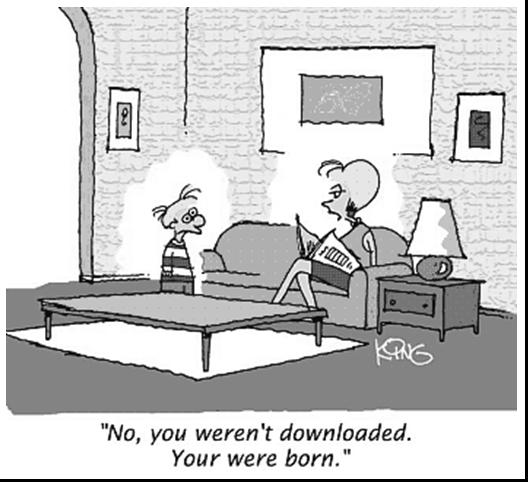
\includegraphics[width=.7\textwidth]{template_modelo_sbc/fig1.jpg}
\caption{Exemplo de estrutura de interface do mural de placas de formatura.}
\label{fig:interface}
\end{figure}

\section{Implementação}

A implementação do sistema foi realizada em arquivos separados para facilitar a
manutenção e reutilização.

\subsection{Gerenciamento de placas}

O arquivo \texttt{mural.js} é responsável pela renderização do mural público. O
script carrega os dados do \texttt{localStorage}, monta os cards das placas e
fornece funcionalidades de edição e remoção. Cada placa inclui campos como
ano/semestre, nome da turma, paraninfo, patrono, formandos e homenagens.

\subsection{Formulário e persistência}

O arquivo \texttt{index.js} gerencia o formulário administrativo em \texttt{home.html}.
O formulário permite incluir imagem por upload ou por URL e valida o preenchimento
obrigatório dos campos antes de salvar. Os dados são gravados no
\texttt{localStorage} em formato JSON.

\begin{table}[ht]
\centering
\caption{Campos principais do cadastro de placas}
\label{tab:fields}
\begin{tabular}{ll}
\hline
Campo & Descrição \\
\hline
Ano/Semestre & Período da turma \\
Reitor/a & Nome do reitor ou reitora \\
Diretor/a do campus & Nome do diretor do campus \\
Coordenador/a & Nome do coordenador \\
Nome da turma & Designação da turma \\
Paraninfo/a & Nome do paraninfo \\
Patrono/Patronesse & Nome do patrono \\
Mestre Amigo & Nome do mestre amigo \\
Professores/as homenageados/as & Lista de professores homenageados \\
Oradora & Nome da oradora \\
Juramentista & Nome do juramentista \\
Formandos & Lista de formandos \\
\hline
\end{tabular}
\end{table}

\subsection{Autenticação}

O sistema utiliza Firebase Authentication em \texttt{login.js} e
\texttt{register.js}. O login valida e-mail e senha, e o cadastro inicial exige
uma chave de administrador para evitar a criação de contas não autorizadas.

\section{Avaliação}

A avaliação do protótipo foi realizada de forma qualitativa, verificando a
execução dos casos de uso principais: visualização de placas, cadastro de nova
placa, edição e exclusão. O protótipo mostra-se funcional e fácil de usar,
embora apresente limitações relacionadas ao armazenamento local.

Entre os principais pontos identificados estão:

\begin{itemize}
  \item o mural permite acesso rápido às informações de formandos e homenagens;
  \item a área administrativa protege as ações de edição e remoção;
  \item o uso de \texttt{localStorage} limita a sincronização entre diferentes dispositivos;
  \item a experiência pode ser melhorada com responsividade e filtros de pesquisa.
\end{itemize}

\section{Conclusão}

Este trabalho apresentou uma solução para o gerenciamento digital de placas de
formatura. O protótipo integra um mural público e um painel administrativo,
utilizando tecnologias web simples e autenticação Firebase para controle de
acesso.

Trabalhos futuros incluem a migração para um banco de dados centralizado,
implementação de armazenamento em nuvem para imagens, aprimoramento da
responsividade e inclusão de recursos de busca e filtragem no mural.

\bibliographystyle{sbc}
\bibliography{tcc_mural_placas}

\end{document}
